\section{App store simulation: AppEco}
\label{sec:analysis_appeco}

An ecosystem has a lot of moving parts and dynamic relationship between the actors inside the ecosystem \cite{Jansen}. One of the ways of studying such relationships is through simulation \cite{castiglione2006agent}.

Lim and Bentley did a comparative analysis of success of different strategies for developers while developing apps for a mobile app store \cite{lim2012successful}. They created a simulation of mobile app store ecosystems called AppEco. In AppEco, developer agents build and upload apps to the app store; user agents browse the store and download the apps \cite{lim2012successful}. They callibrate AppEco with suitable parameters that resembles the Apple's App Store and investigate the result by evaluating different developer strategies in terms of downloads received, app diversity and adoption rate.

We further explain the features of AppEco from \cite{lim2012successful} in the following section because they are relevant for our own simulation discussed in Chapter~\ref{chap:design}.

\subsection{AppEco Components}

In AppEco there are three components: apps, developers and users. In a real app ecosystem these three components form complex relationships, filling niches, competing and cooperating similar to a biological ecosystem \cite{lin2009operating}. In AppEco, apps, developers and users are abstracted models of their real world counterpart. Developer and user models are artificial life agents with certain behaviors. They are described below:

\subsubsection*{Developers}
\label{subsubsec:appeco_components_developers}

A developer agent takes $devDuration$ days to build an app and then uploads it to the app store. Developer keeps track of all of the apps she has developed. She uses one of the following strategies to build apps:

\begin{itemize}
  \item \emph{S0 Innovator} builds an app with random features each time.
  \item \emph{S1 Milker} try to milk an idea repeatedly. She makes an app and copies it with slight variations to produce many different apps.
  \item \emph{S2 Optimiser} makes variations in own best app each time. The strategy models developers who learn from their downloads and want to improve.
  \item \emph{S3 Copycat} copies app from the Top App Chart. The strategy models less creative developers but who want to achieve many downloads quickly.
  \item \emph{S* Flexible} begins with a strategy S0-S3. Each developer than has a 0.99 probability to pick an app from the Top App Chart list and to change the strategy to be the same as the developer of the selected app.
\end{itemize}

\subsubsection*{Apps}
\label{subsubsec:apps}

An App is developed and uploaded by the developer to the app store. Lim and Bentley show a novel way to model the different natures of an app by using a 10x10 feature grid.

\begin{figure}[!htb]
  \centering
  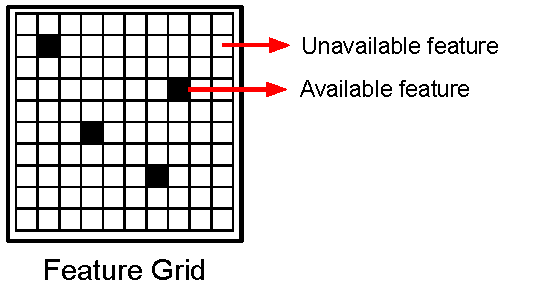
\includegraphics[width=9cm]{figures/example_service_grid.pdf}
  \caption{A grid representing an App. Black cells represent features and white cells represents lack of features. The coordinate of a cell represents its uniqueness.}
  \label{fig:example-grid}
\end{figure}

As shown in Figure~\ref{fig:example-grid}, a 10x10 grid can have white and black cells. A white cell is an empty cell and a black cell is filled cell. Each cell represents a unique feature identified by its x and y coordinates. In the figure, 4 of 100 cells filled, meaning the grid contains 4 out of 100 possible features. 

How each cell of the grid is filled depends upon the strategy of the app developer. We explain them below:

\begin{itemize}
  \item \emph{S0:} Each cell in the grid of the app is filled probabilistically. The probability of a cell being filled is given by $P_{Feat}$, one of the parameters for simulation calibration.
  \item \emph{S1:} For the first app, S1 also fills the cells as done by S0. For any further app, S1 copies the existing features of her first app and introduces random mutation. Mutation is explained below.
  \item \emph{S2:} For the first app, S2 also fills the cells as done by S0. Then the new apps are developed by copying features from her most successful (popular) app and introducing random mutation to it.
  \item \emph{S3:} One of the apps is randomly selected from the Top Apps Chart and its features are copied with random mutation.
\end{itemize}

The probability that a developer will mutate an app when copying is 0.5. During mutation, a developer picks one of the filled cells and moves its location to an empty cell.

\begin{figure}[!htb]
  \centering
  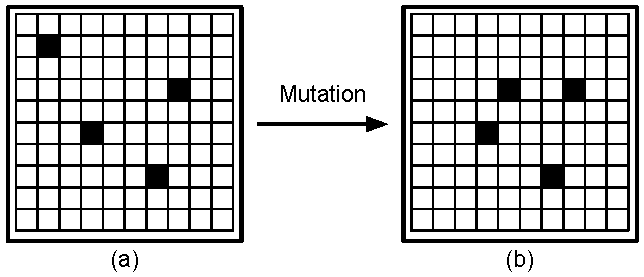
\includegraphics[width=9cm]{figures/example_app_grid_mutation.pdf}
  \caption{Example of grid mutation: One of the cells is randomly picked from (a) and moved to another location in (b).}
  \label{fig:example-grid-mutation}
\end{figure}

\subsubsection*{Users}

A user agent in AppEco downloads apps uploaded in the app store. The behavior of a user in AppEco is modelled as following:

\begin{itemize}
  \item Each user has a preference of what features she likes in her apps. The preference is also modelled using a grid (preference grid) as shown in Figure~\ref{fig:example-grid}. User agents use different probability $P_{Pref}$.
  \item Each filled cell in a preference grid represents a feature the user desires.
  \item If all the filled cells of the app grid are also filled in the preference grid of a user, the user downloads the app.
  \item A user keeps track of all the downloaded apps.
  \item A user takes a break of certain days before browsing the app store again for new apps. The number of days $daysBtwBrowse$ for each user is randomly selected between $[bro_{min}, bro_{max}]$ whose values are selected as part of simulation calibration.
\end{itemize}

\subsection{Algorithm}

The AppEco algorithm is responsible for modelling the interaction between the AppEco components mentioned in the section above. Each timestep in the algorithm represents a single day.

The population of developer and user agents grow following a sigmoid curve. The sigmoid curve follows the population growth as described in ecological studies given by Eq.~\ref{eqn:appeco_population_growth} \cite{lim2012successful}.

\begin{equation}\label{eqn:appeco_population_growth}
  pop_t=MinPop+\frac{MaxPop-MinPop}{1+e^{S*t-D}}
\end{equation}

Where, 
$pop_t  =$ the size of the population,
$MinPop =$ the minimum population,
$MaxPop =$ the maximum population,
$S =$ constant that determines the slope of the growth curve,
$D =$ constant that shifts the curve from left to right.


\begin{figure}[!htb]
  \centering
  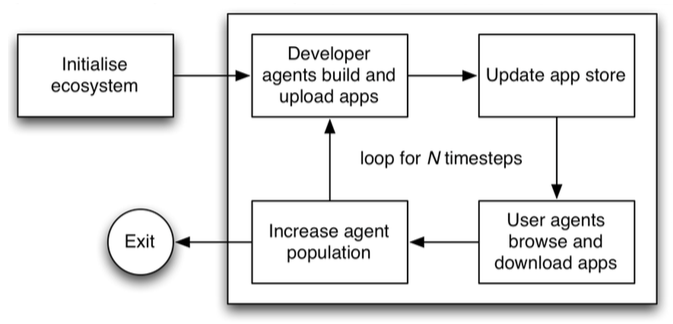
\includegraphics[width=11cm]{figures/appeco_algorithm.png}
  \caption{AppEco algorithm (Source:~\cite{lim2012successful}).}
  \label{fig:appeco-algorithm}
\end{figure}

The algorithm of AppEco is shown in Figure~\ref{fig:appeco-algorithm}. These steps are briefly described in the following section:

\subsubsection*{Initialize ecosystem}

The first step of AppEco is to initialize the system with timestep $t=0$. Most app stores have some apps before they launch to public. AppEco creates an initial number of app artefacts. AppEco also contains a pool of initial developers with all the strategies S0, S1 and S2 (S3 cannot start at $t=0$ because the Top Apps Chart is not ready yet). The initial app artefacts are assigned randomly to the initial pool of developers.

\subsubsection*{Developer agents build and upload apps}

For each day, active developers (subset of all developers) are selected based their $devDuration$. Each active developer uploads an app to the app store. Each developer then becomes inactive for the next $devDuration$ number of days before uploading another app. Developers can also become inactive based on probability $P_{Inactive}$.

\subsection*{Update app store}

In AppEco, the app store contains two charts:

\begin{enumerate}
  \item \emph{New Apps Chart} which includes the newest apps uploaded by users.
  \item \emph{Top Apps Chart} which includes the best ranked apps among all apps.
\end{enumerate}

For \emph{New Apps Chart}, any newly uploaded app has a probability $P_{OnNewChart}$ chance of appearing on it. There are maximum $N_{MaxNewChart}$ number of apps in the chart. Both variables are part of simulation calibration.

For \emph{Top Apps Chart}, the formula given by Eq.~\ref{eqn:appeco_app_ranking} is used to calculate the ranking of each app.

\begin{equation}\label{eqn:appeco_app_ranking}
rank = 8*D_1 + 5*D_2 + 5*D_3 + 3*D_4
\end{equation}

Where, $D_n$ is the number of downloads received by an app on the $n$th day before current day.
Like \emph{New Apps Chart}, there is a limit to the number of apps listed in \emph{Top Apps Chart} given by $N_{MaxTopChart}$.

\subsection*{User agents browse and download apps}

For each day, active users (subset of all users) are selected based on their $daysBtwBrowse$. Each of the active users browses the \emph{New Apps Chart} and \emph{Top Apps Chart} for the current day and downloads apps that match her preference grid. 

Users are also likely to search for a particular app based on their own requirements. Search however is simulated such that a random list of apps are shown to the user. The user then uses the same method as with the two charts described previously and downloads according to her preference. 

After download, each user waits for another $daysBtwBrowse$ number of days before becoming active and downloading another set of apps.

\subsection*{Increase agent population}

To simulate the growth of the ecosystem, the number of users and developers are increased for the next timestep using Eq.~\ref{eqn:appeco_population_growth}.

Each new developer is assigned $devDuration$ and each new user is assigned $daysBtwBrowse$ as explained previously.

\subsection{Simulation Results}

AppEco was calibrated using values for probability variables and other constants such that the growth of users, developers, apps and downloads matched the trend of the Apple's App Store. The total simulation was run for 1080 timesteps (3 years, 1080 days on average with 30 days per month). 

They give the following results:

\textbf{C1} According to AppEco, they found out that Copycat strategy S3 was the most successful with highest average downloads, top 20 downloads and top 20 average downloads \cite{lim2012successful}. Lim and Bentley back up the claim by giving example that when the app \emph{Angry Birds} was popular, the copycats had parasitised the app with clone of the app that successfully rose to the Top Apps Chart.

\textbf{C2} They claim that Innovator strategy produced the diverse apps fulfilling maximum users' preference for apps \cite{lim2012successful}.

\textbf{C3} They finally claim that S2 Optimiser strategy enables the developer to become more successful as they develop more apps although Copycat strategy is a winner in terms of number of downloads \cite{lim2012successful}. This is because copycats are plagiarising the work of other developers which eventually gets punished by the app store. The S2 Optimiser strategy produces an enhanced version of their apps which resembles the improvement developers make in real world by listening to user feedbacks.

Readers can refer to \cite{lim2012successful} for further interesting results from AppEco.

\subsection{Conclusion}

The AppEco simulation provides valuable insights to the nature of developers and users. Their results show which strategy are successful in terms of popularity, earnings and diversity. The also give valuable examples in real world that match their results.

The AppEco simulation is the first artificial life model of mobile application ecosystems \cite{lim2012successful}. The AppEco simulation presents a base example for doing further simulations on app stores.

The concept of grids is novel and can be applied to other entities where each entity can be compared to other entities in terms of similarities and differences. I.e., two grids having exactly the same number of filled cells in exactly same coordinates are equal and otherwise different. Grids also allow entities to undergo changes over time by mutation. Finally, grids allow to express complexity of entities based on the number of filled and unfilled cells.

AppEco uses a lot of random processes with different probability distributions during simulation. But with suitable calibration, it shows that through simulation, results can be achieve that mimic the results of a real life app store. This shows the suitability of the algorithm of AppEco.

In Section~\ref{sec:s2store_ecosystem} we describe the \emph{S2Store Ecosystem} which has elements similar to the one described here. In Section~\ref{sec:s2eco} we describe a simulation for S2Store Ecosystem based on AppEco.

